\subsection{Faults, Errors, and Failures}
\label{sec:terminology}
The usage of the terms error, failure, and fault are defined in ARP4754A~\cite{SAE:ARP4754A} and are described here for ease of understanding. A \textit{failure} is an event that occurs when the delivered service of a system deviates from correct behavior. A service of a system is a sequence of the system's external states. This means that if a service failure occurs, one or more of the systems external states has deviated from the correct service state. This deviation is called an \textit{error}. The complete definition of an error is the part of the state of the system that may cause a failure. Not all errors will affect the external state of a system and cause an failure. The cause of an error is a \textit{fault}. Faults can be \textit{active} or \textit{dormant}. A fault is active when it causes an error to occur, else it is dormant.

\iffalse
\begin{figure*}
	%\vspace{-0.956in}
	\centering
	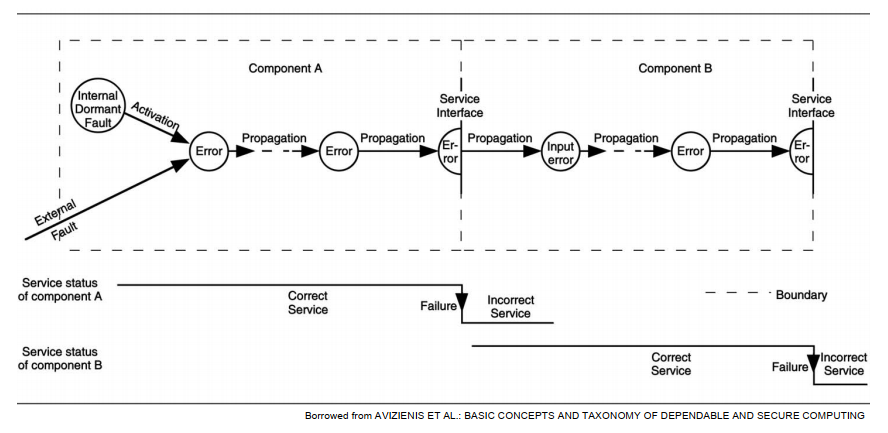
\includegraphics[width=1.0\textwidth]{images/fault_error_failure.png}
	%\vspace{-0.4in}
	\caption{Faults, Errors, and Failures}
	\label{fig:fault_error_failure}
\end{figure*}
\fi

The relationship between faults, failures, and errors were summarized by Aviyienis, et. al.~\cite{basicConcepts} and are described here once again.% and is shown in Figure~\ref{fig:fault_error_failure}.

\begin{itemize}
\item A fault is active when it causes an error. An active fault can be an internal fault that was previously dormant but has been activated or it can be an external fault. Fault activation is what causes a dormant fault to become active. 

\item Error propagation in a component is caused by the computation process of that component. In this process, an error is successfully transformed into other errors. Error propagation from component A to component B occurs when an error reaches the service interface of component A. The service delivered from component A to component B is no longer correct and thus the error is propagated into component B through the interface between the two components.

\item A service failure occurs when that error is propagated to the service interface and causes the service of the system to be incorrect. The failure of a component causes a fault in the system that contains the component. Service failure of a system will cause external fault(s) for the other systems that recieve service from the given system. 
\end{itemize}